\documentclass{article}

\usepackage[utf8]{inputenc}
\usepackage{hyperref}
\hypersetup{
    colorlinks=true,
    linkcolor=blue,
    filecolor=magenta,      
    urlcolor=cyan,
}

\title{Udacity Machine Learning Nanodegree\\
       Capstone Project Report \\
        \ \\
        Predicting Swimming Pool Occupancy}
\author{Lukas Koucky}
\date{9 January 2020}

\usepackage{natbib}
\usepackage{graphicx}
\usepackage{amsmath}

\begin{document}

\maketitle

\section{Definition}
\subsection{Project Overview}
I started swimming regularly in my local swimming pool \href{https://www.sutka.eu/en/}{\v{S}utka swimming pool} about two years ago. Usually when I’m leaving work I ask myself a question: ''Should I go swimming today?'' I can look at the web page of swimming pool to see how many visitors are in the pool right at that moment to get a hint if the swimming lines are reasonably occupied or overcrowded. But the problem is that it takes me another 45 minutes to get the pool during which the situation can change a lot. But what if I have a tool that will predict how many people will be in a pool when I get there or even tell me in the morning if today is a good day to visit the pool let’s say between 5PM and 6PM? Goal of this capstone project was to develop such tool. \par

Predicting number of people in pool throughout the whole day is typical example of time series forecast. In this project more precisely multivariate time series prediction. In simple or univariate time series prediction models input is single series of observations and output is series of future predictions (i.e. number of visitors in the pool). On the other hand multivariate time series prediction produces the same output as univariate one but each input timestamp have multiple observations or features. In this project not just attendance data are the input for prediction algorithm but also number of reserved swimming lines, weather or public holidays at each time step. These problems are studied in both academic and professional sphere for example for financial market predictions \footnote{\url{https://arxiv.org/abs/1909.12789}}, attendance prediction \footnote{\url{https://www.ncbi.nlm.nih.gov/pmc/articles/PMC6109553/}}, power consumption prediction \footnote{\href{https://machinelearningmastery.com/how-to-develop-lstm-models-for-multi-step-time-series-forecasting-of-household-power-consumption/}{https://machinelearningmastery.com/household-power-consumption}} or air pollution prediction \footnote{\url{https://www.kaggle.com/c/dsg-hackathon}} and many many more.\par

\subsection{Problem Statement} \label{sec:problem_statement}

There were two main goals for this project. First one was to train and deploy machine learning system that will be able to predict number of visitor in \v{S}utka swimming pool throughout the day and the second was to create web page that can visualise predicted occupancy (number of visitors) at any time of the day using the trained model. To fulfill both tasks following was done:

\begin{itemize}
\item Gather all relevant data for machine learning algorithms
\begin{itemize}
\item Historical data with number of pool visitors throughout the day are the most important data source for this task. But there are many more data inputs apart from historical data of swimming pool attendance that could be relevant for training of machine learning algorithms. For example weather or number of reserved swimming pool lines. First task was to discover all possibly useful data sources and gather all data.
\end{itemize}

\item Clean and preprocess data into useful format
\begin{itemize}
\item There are usually some errors in gathered data. Sometimes the webserver collecting occupancy data experience problems, sometimes webpages of pool are not accessible and these data points must be removed. There are also other possible situations where input data are not suitable for machine learning - for example days when pool was closed due to cleaning or holidays and attendance was therefore zero. 
\item Other preprocessing steps like normalization, one hot encoding of some features and generating new features
\item Export to CSV and pickle format for easier processing
\end{itemize}

\item Train 3 different machine learning algorithms for pool occupancy prediction on clean data
\begin{itemize}
\item Several machine learning algorithms was inspected and trained for the task of prediction pool occupancy. 
\item Following algorithms were inspected: Monthly average, Gaussian Mixture Model, Hidden Markov Model, Long Short Term Memory, Convolutional Neural Networks, Support Vector Machine, AdaBoost, Random Forest Classifier, Extra Trees Classifier
\item For supervised learning algorithms was time series transformed using sliding windows approach described in \citep{brownlee2019howtosupervised}.
\end{itemize}

\item Create web page that will visualize predictions of machine learning algorithms and inform user when is the good time to visit the pool for selected day
\begin{itemize}
\item Models trained in previous step were deployed and used for actual prediction on a web page that visualize prediction for selected day and offers possibility to compare results of multiple algorithms
\end{itemize}
\end{itemize}

\begin{figure}[h!]
\centering
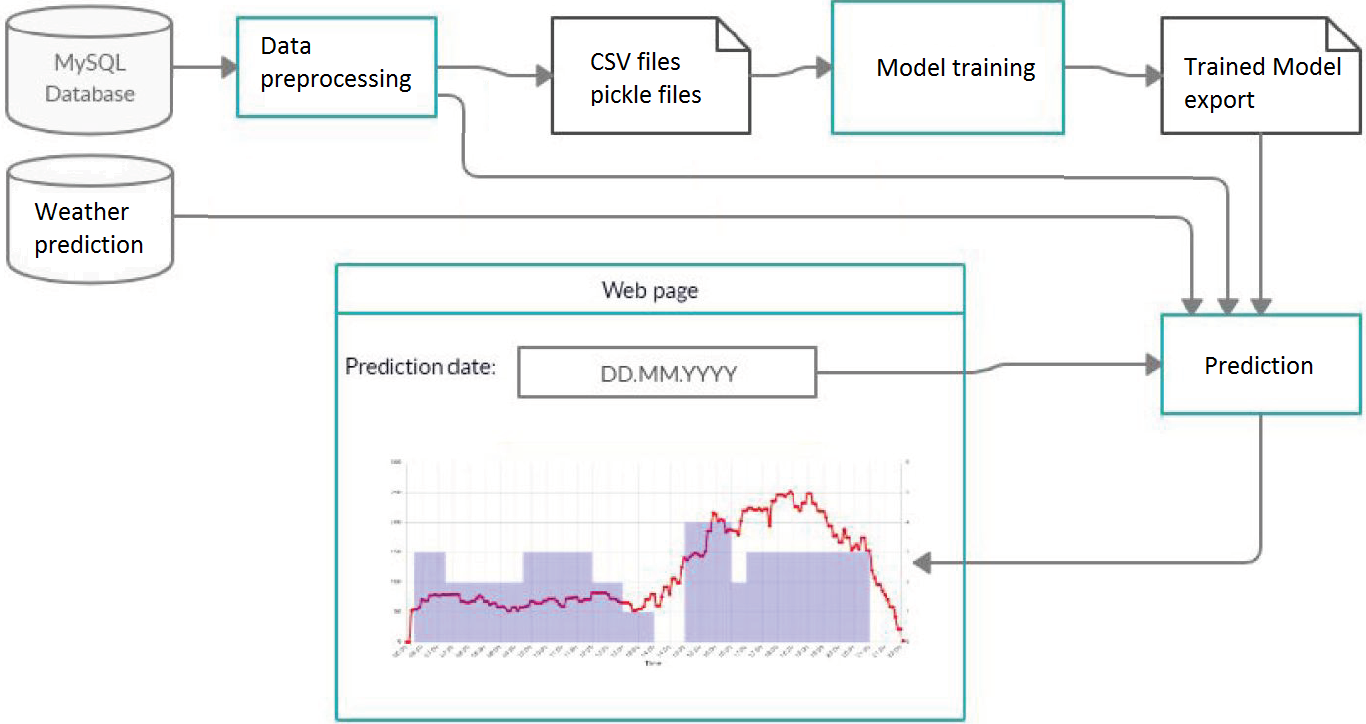
\includegraphics[width=12cm]{imgs/project_pipeline}
\caption{Diagram of project pipeline}
\label{fig:diagram_pipeline}
\end{figure}

\subsection{Metrics}
Mean squared error is used to measure performance of prediction. Predictions are always generated for the whole day so it makes sense to measure performance also on the whole day. 

\begin{equation}
\label{eq:mse}
MSE_{day}(y,\hat{y}) = \dfrac{1}{n} \sum^{n-1}_{i=0}(y_i-\hat{y}_i)^2
\end{equation}

Mean square error of one day's prediction is computed using Equation \ref{eq:mse} above where $y$ is vector of ground truth data (real attendance during the whole day with 5 minute sampling). $\hat{y}$ is vector of predicted attendance in the same time steps as $y$. $n$ is number of time steps for the whole day (usually 288). $y_i$ is the $i$-th sample in vector $y$. 

The performance of implemented algorithms will be measured as a mean of $MSE_{day}$ on all days in testing dataset. This metric will show which algorithm performs better overall.

\begin{equation}
\label{eq:mse_all}
MSE_{dataset} = \dfrac{1}{k} \sum^{k-1}_{day=0}MSE_{day}(y,\hat{y})
\end{equation}

Where $k$ is the number of days in dataset. $y$ is vector of ground truth data for given $day$ and $\hat{y}$ is vector of predicted attendance for given $day$.


\color{red}
TODOs:
\begin{itemize}
    \item Prepsat jake algoritmi byly prozkoumane aby to odpovidalo v Train 3 different machine learning algorithms...
\end{itemize}
\color{black}

\section{Analysis}
\subsection{Data Exploration} \label{sec:data_exploration}
\color{red}
TODOs:
\begin{itemize}
    \item Analyze the problem through visualizations and data exploration to have a better understanding of what algorithms and features are appropriate for solving it.
    \item Only few organisations are used, describe why
    \item Unusual data
    \item Weekend vs weekday
    \item Image2 - histogram of how often the organization is present
    \item Image3 - interesting organisation and why to use them 
    \item Data preprocessing, divide into days
    \item If a dataset is present for this problem, have you thoroughly discussed certain features about the dataset? Has a data sample been provided to the reader?
    \item If a dataset is present for this problem, are statistics about the dataset calculated and reported? Have any relevant results from this calculation been discussed?
    \item If a dataset is not present for this problem, has discussion been made about the input space or input data for your problem?
    \item Are there any abnormalities or characteristics about the input space or dataset that need to be addressed? (categorical variables, missing values, outliers, etc.)

\end{itemize}
\color{black}

Every machine learning project starts with the data gathering and analysis. Data for this project comes from several sources. The most important data input is collected on my personal webserver that stores pool occupancy every 5 minutes into the MySQL database from publicly available data on \v{S}utka pool web page. Data are collected for past 2 years which means I have more than enough data for training, validation and testing of machine learning algorithms. But there are also many other inputs that influence attendance of swimming pool and are highly valuable for predictions. One of the most important is number of reserved swimming lines with names of organisations reserving the lines. This information is also collected from publicly available data on \v{S}utka pool web page. Next important input is time of the year that is included in timestamp of each timesample, public holidays acquired from \href{https://www.officeholidays.com/countries/czech-republic}{officeholydas.com} and finally local weather acquired from archive of \href{https://www.in-pocasi.cz/archiv/}{in-pocasi.cz}. Local weather contains information about temperature, humidity, precipitation, wind strength and air pressure from multiple stations across Prague. All these information are also stored in the MySQL database. You can find sample export from database in attached file database\_sample.txt and description of all tables and columns in file database\_description.pdf. History weather information is collected in database but for the occupancy prediction into the future is  used \href{http://www.in-pocasi.cz/pocasi-na-web/}{in-pocasi.cz} free predictions REST API. Working directly with MySQL database would not be very comfortable. This is why the database was exported, preprocessed and saved to csv files and pickle files. More about preprocessing can be found in section \ref{sec:data_preprocessing}. 

\begin{figure}[h!]
\centering
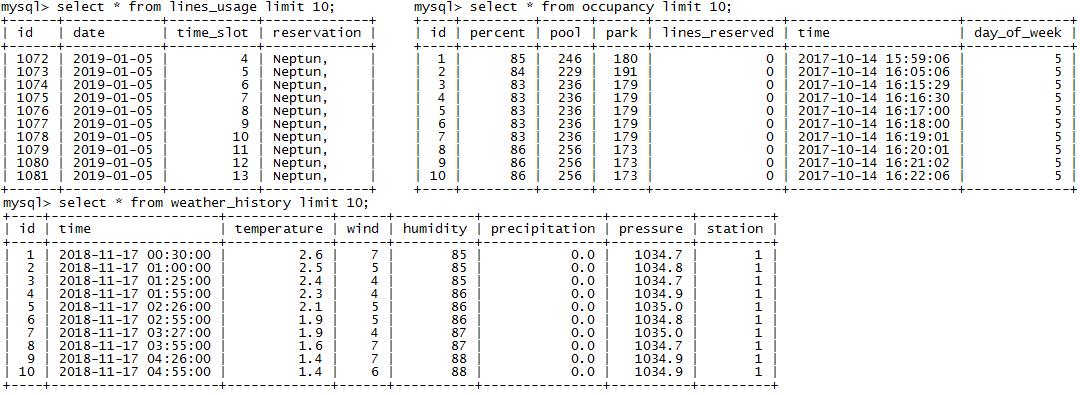
\includegraphics[width=12cm]{imgs/db_export.png}
\caption{Sample export of 10 rows from all tables in MySQL database. Top left table \emph{lines\_usage} with information about which organisation reserved line in given time. Top right table \emph{occupancy} with information about number of people in the pool. Bottom table \emph{weather\_history} with information about weather history in Prague.}
\label{fig:db_export}
\end{figure}

\subsubsection{Pool attendance data}
Attendance data are stored in table \emph{occupancy}. Data are collected every 5 minutes which results in 288 time samples from each day. As you can see on Image \ref{fig:db_export} top right there are more than just pool attendance stored for each time stamp. Following information are store in this table:
\begin{itemize}
    \item \textbf{id} - unique identifier integer of data sample.
    \item \textbf{percent} - occupancy of pool in percentage. 100 means that pool is full. 
    \item \textbf{pool} - number of people in the pool area.
    \item \textbf{park} - number of people in the park area.
    \item \textbf{lines\_reserved} - not used any more, set to 0. Number of reserved lines together with additional information are stored in table lines\_usage described in section \ref{sec:lines_usage}.
    \item \textbf{time} - timestamp with date and time.
    \item \textbf{day\_of\_week} - day of week starting with 0 for Monday.
\end{itemize}

Notice that there are number of people in pool and in park. This is because the whole \v{S}utka pool is divided into two parts. First part is pool with 50 meters swimming pool, small pool for little children, showers, two steam rooms, two saunas and resting area. Second part is park with small water park (water slides, whirlpools, outdoor relax area, foot court and bar). These two parts of the pool are connected with tourniquets so the number of people in each area is precisely monitored. Since only prediction of number of people in pool is the scope of this project columns \emph{percent} and \emph{park} are not used. Also \emph{lines\_reserved} is not used since this information is stored in separate table \emph{lines\_reserved}.

\subsubsection{Lines usage data} \label{sec:lines_usage}
Table \emph{lines\_reserved} stores information about reserved lines. Reservations can be made for 15 minutes time slots and each organisation can reserve more than one line for any number of time slots. Therefor names of the organisations and number of lines in each time slot are stored. If there is no entry for particular day or time it means that no line is reserved. Since only time slot and names of organisations that rents line in particular time slot is saved there is no information about which lines precisely are booked - only how many lines are booked. But it is not necessary to know which specific line was reserved to predict attendance, information about organisation and number of lines is sufficient. Description of table columns is following:
\begin{itemize}
    \item \textbf{id} - unique identifier integer of data sample
    \item \textbf{date} - date in format YYYY-MM-DD
    \item \textbf{time\_slot} - integer from 0 to 63 that represents time slot of swimming line reservation in reservation table on \href{https://www.sutka.eu/en/obsazenost-bazenu}{\v{S}utka swimming pool web page}
    \item \textbf{reservation} - comma separated strings containing names of clubs or organisations that rented the line. One name can be represented multiple times which means that given organisation rented multiple swimming lines
\end{itemize}

\subsubsection{Weather data}
Table \emph{weather\_history} stores historical data of weather in Prague. Data are collected from \href{https://www.in-pocasi.cz/archiv/}{in-pocasi.cz archive}.There are several measurement stations
available each with the unique id in column station. Description of table columns is following:
\begin{itemize}
    \item \textbf{id} - unique identifier integer of data sample
    \item \textbf{time} - timestamp with date and time
    \item \textbf{temperature} - temperature in degrees of Celsius
    \item \textbf{wind} - wind strength in meters per second
    \item \textbf{humidity} - humidity in percents
    \item \textbf{precipitation} - rain or snow precipitation in millimeters
    \item \textbf{pressure} - air pressure in kPa
    \item \textbf{station} - unique id of weather station where the measurement comes from
\end{itemize}

\subsection{Exploratory Visualization}
\begin{figure}[h!]
\centering
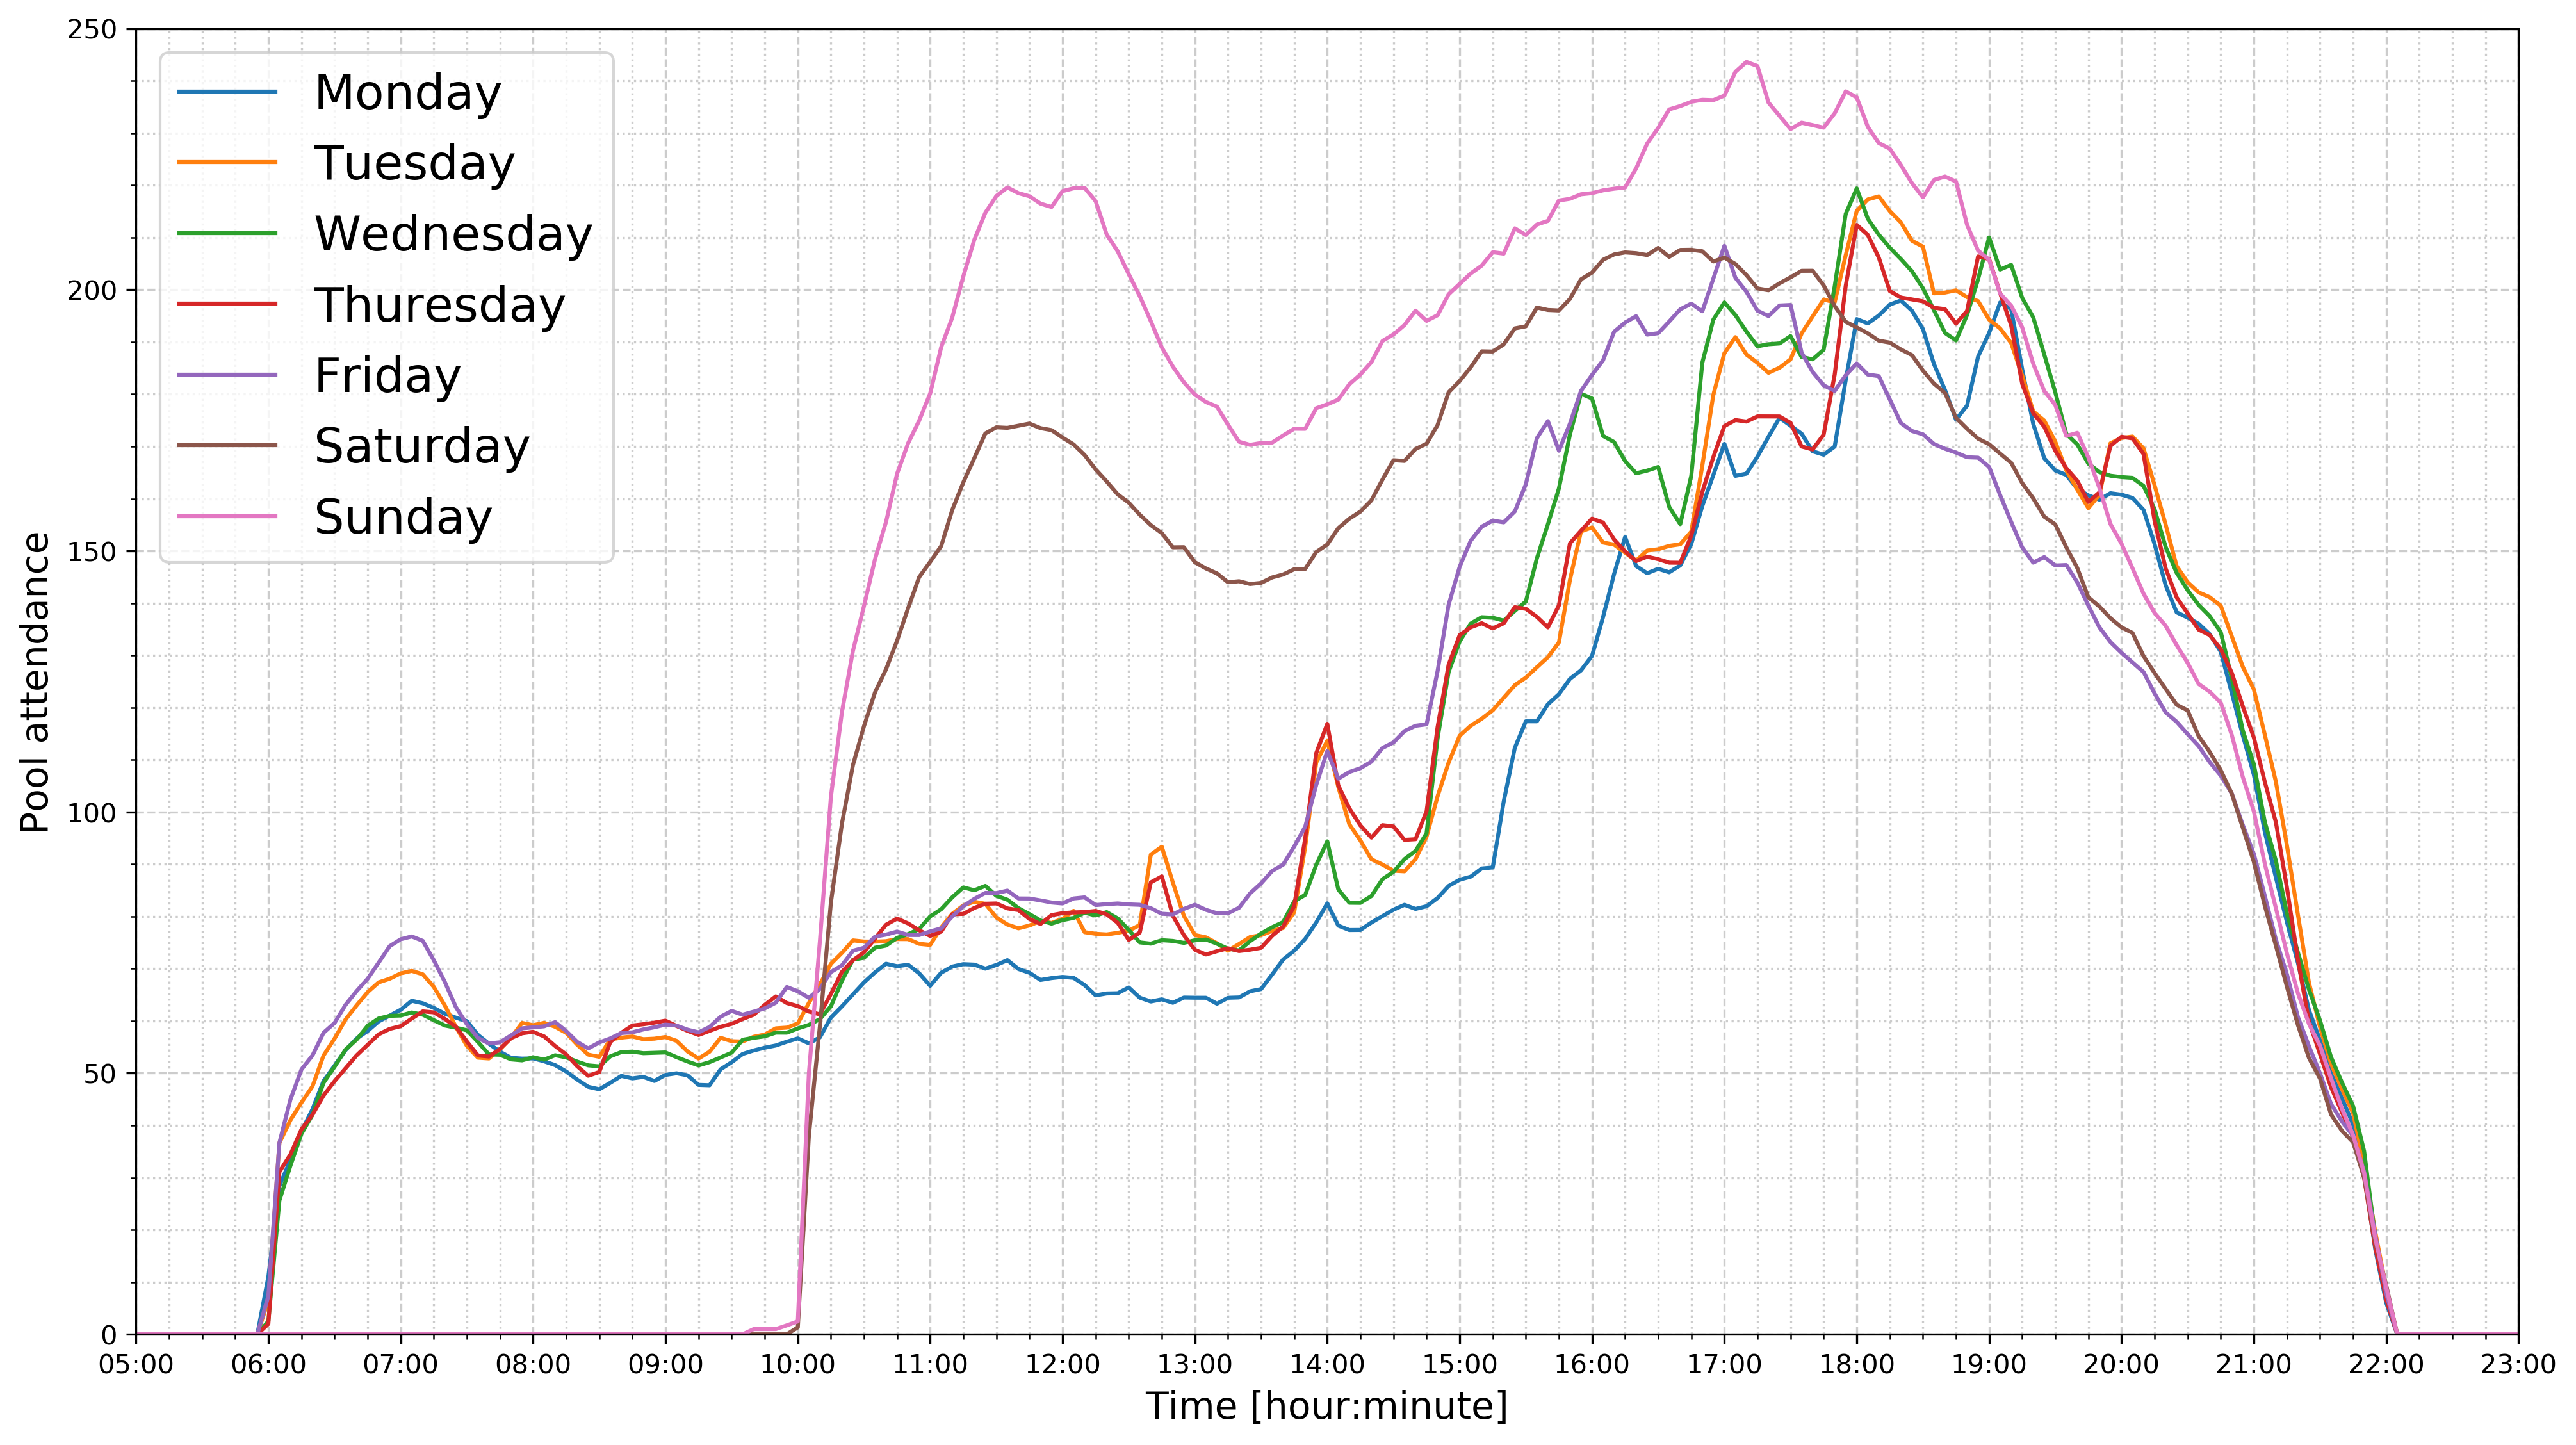
\includegraphics[width=12cm]{imgs/averages}
\caption{Average attendance for each day of week}
\label{fig:averages}
\end{figure}

\begin{figure}[h!]
\centering
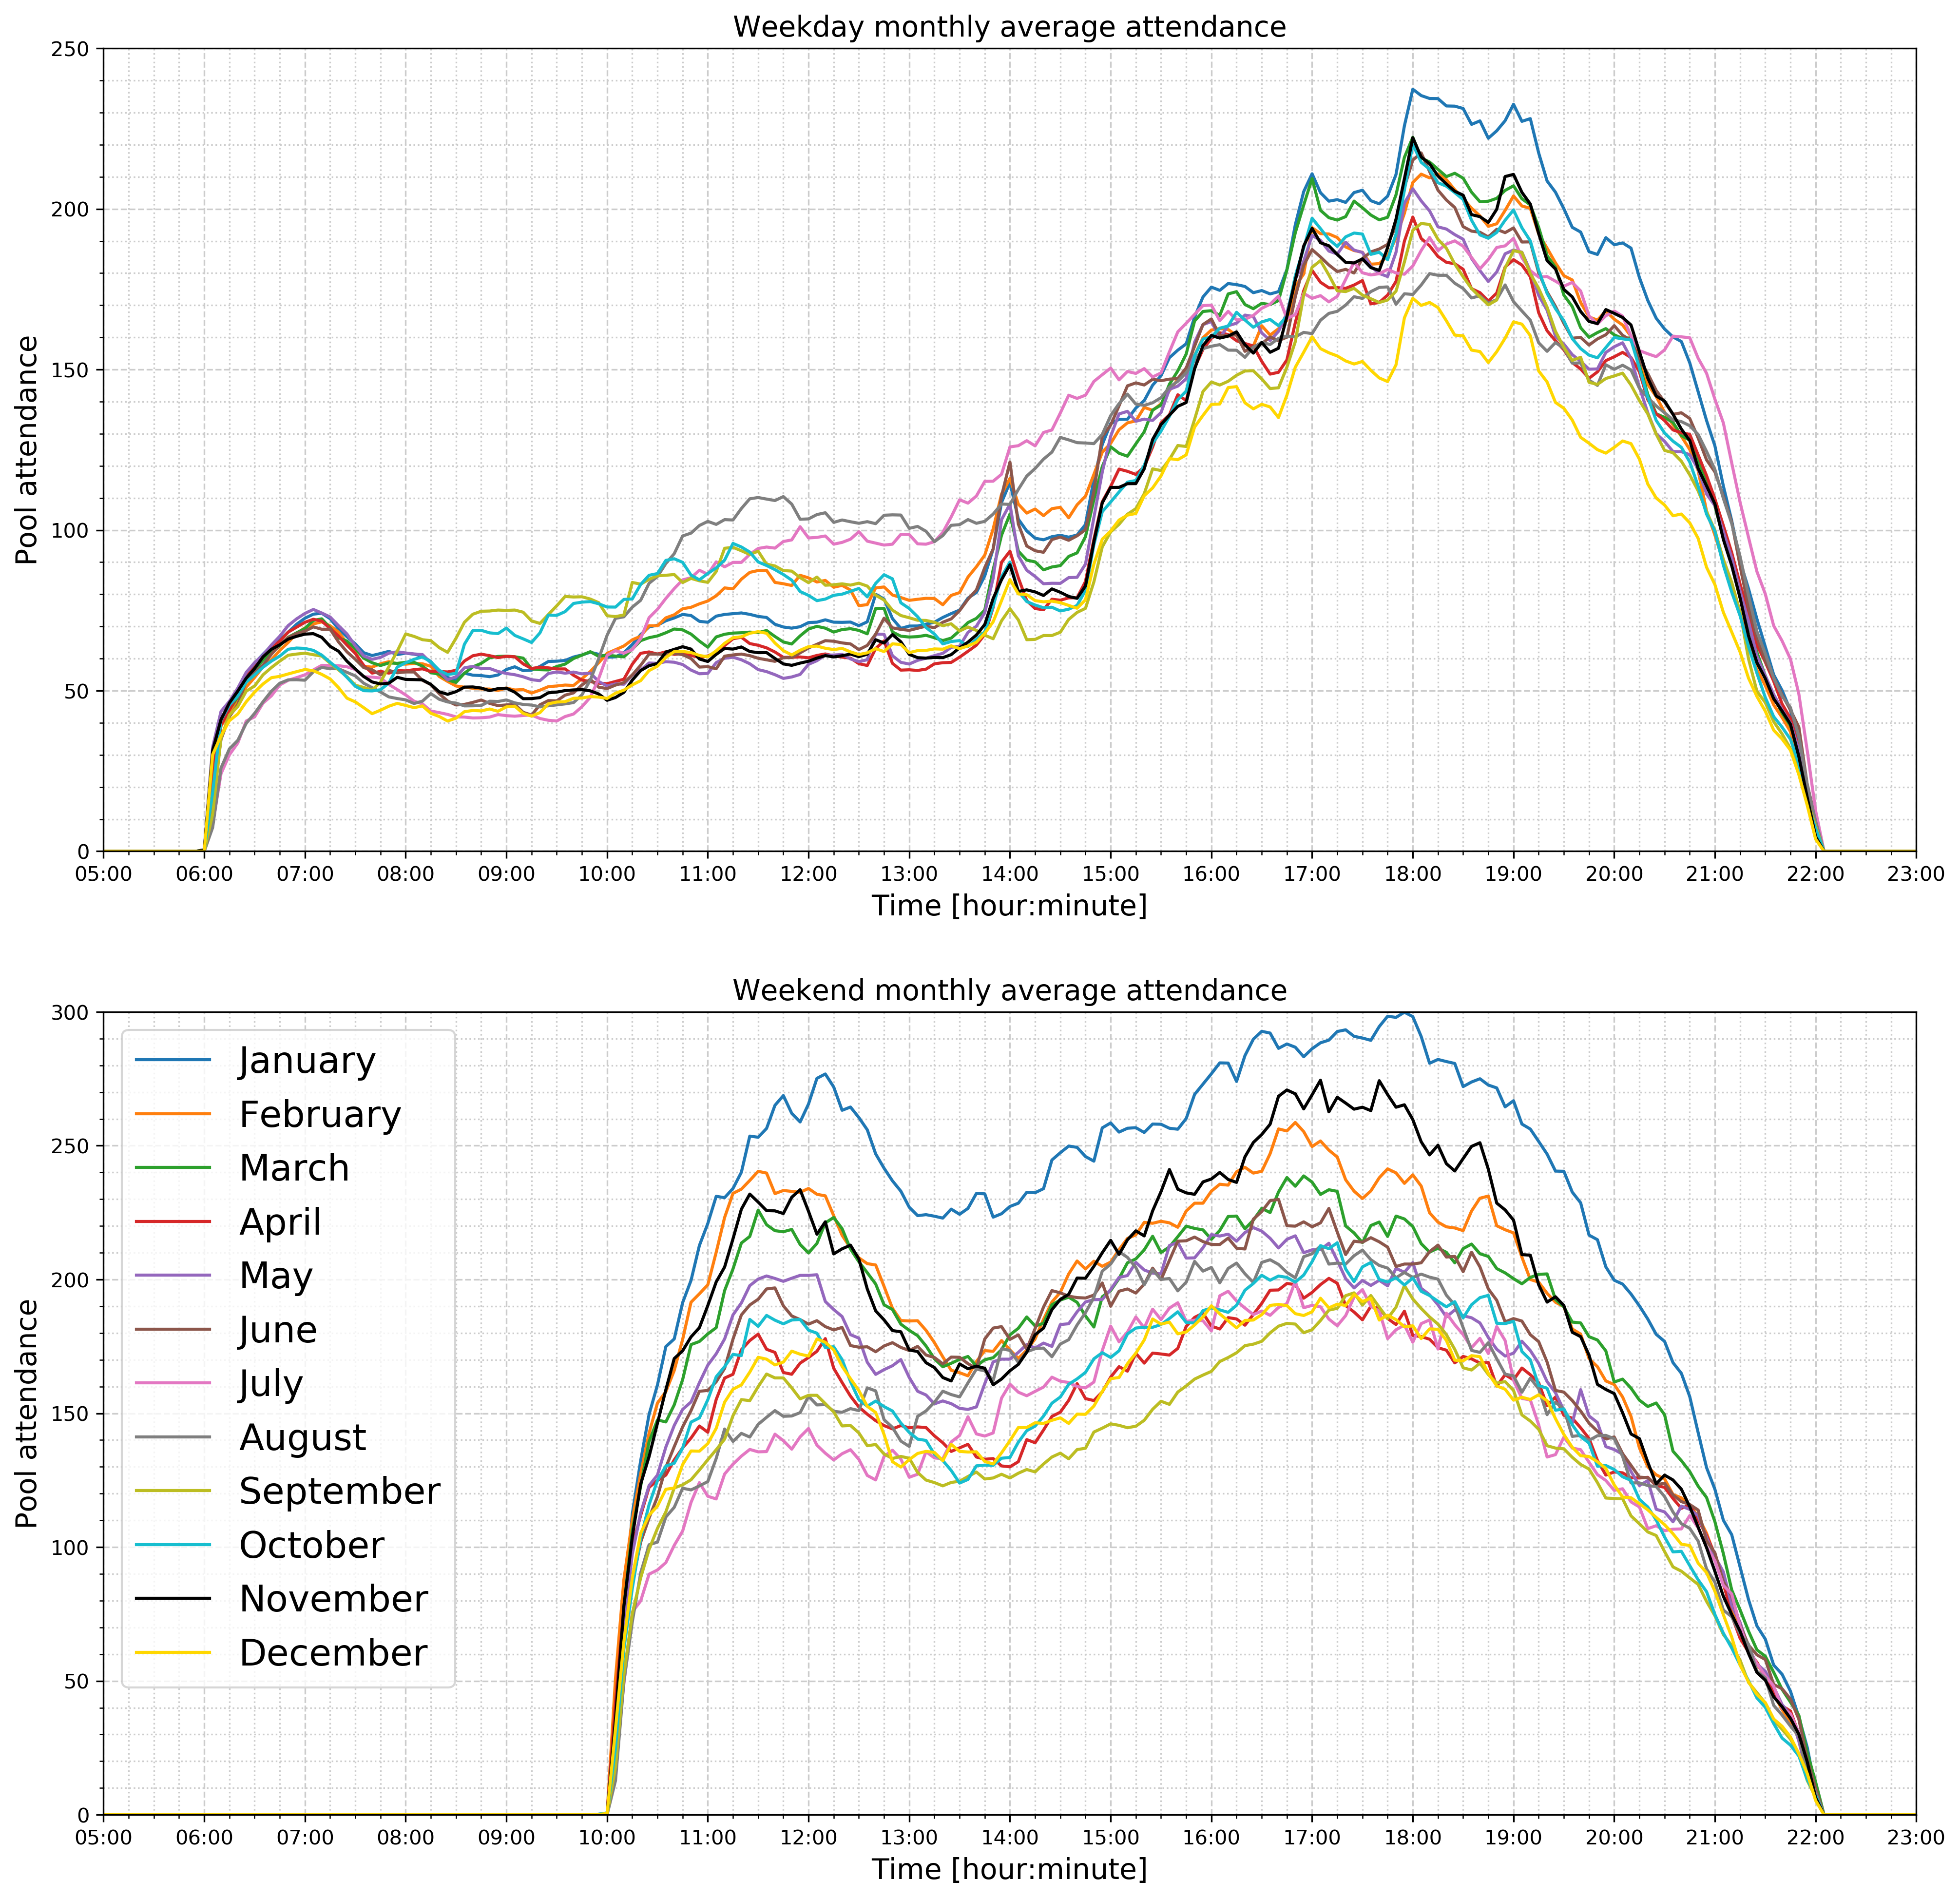
\includegraphics[width=12cm]{imgs/monthly_averages_together.png}
\caption{Monthly average attendance.}
\label{fig:monthly_averages}
\end{figure}

\color{red}
TODOs:
\begin{itemize}
    \item Have you visualized a relevant characteristic or feature about the dataset or input data?
    \item Is the visualization thoroughly analysed and discussed?
    \item If a plot is provided, are the axes, title, and datum clearly defined?
\end{itemize}
\color{black}   


Image \ref{fig:averages} shows average attendance for each day of week. This image shows several important patterns in data. Most obvious is difference between weekend and weekday. On weekdays is pool open from 6:00 and attendance quickly rise to 50 people. Than from around 14:00 attendance rise until 18:00 when it starts to drop again until closing time at 22:00. On weekend days pool opens at 10:00 which is followed by steep increase of occupancy that drops a little around 12:00, then rise again and from 18:00 decrease until closing time at 22:00.

\subsection{Algorithms and Techniques}
\color{red}
TODOs:
\begin{itemize}
    \item Are the algorithms you will use, including any default variables/parameters in the project clearly defined?
    \item Are the techniques to be used thoroughly discussed and justified?
    \item Is it made clear how the input data or datasets will be handled by the algorithms and techniques chosen?
\end{itemize}
\color{black}

\subsubsection{Random Forest Classifier}
Random Forest Classifier is an ensemble method that combines multiple decision trees. Each decision tree produces prediction and the most frequent prediction is chosen as the output of Random Forest Classifier. Randomness in name comes from random bagging during learning phase. Each decision tree is learned on different subset of training data generated by randomly sampling the training set. Also the decision at each node is made on random sub-sample of available features and the best split is used \citep{yiu2019randomforest} \citep{wiki2019randomforest}.


Since Random Forest is a supervised learning method sliding windows approach described in \citep{brownlee2019howtosupervised} was used to serve data. At each time stamp are all other available features provided. This creates vector of input features with following content:
\begin{equation}
\label{eq:input_vector}
v(t) = (attendance(t), lines(t), minute(t), day, month, year, weather(t), org(t))
\end{equation}

Where 
\begin{itemize}
    \item $t$ is the time step of the day. Each day is sampled with 5 minute steps. So for example $t = 0$ is time 0:00, $t = 3$ is time 0:15 and $t = 287$ is time 23:55, 
    \item $v(t)$ is vector of features at time $t$.
    \item $attendance(t)$ is pool attendance at time $t$.
    \item $lines(t)$ is number of reserved lines at time $t$.
    \item $minute(t)$ is minute of the day at time $t$. Minute of the day is counted from the beginning of the day.
    \item $day$ is the day of week indexing from 0 as Monday. So for example 1 is Tuesday and 6 is Sunday.
    \item $month$ is the month of the year indexing from 0 as January. So for example 3 is April and 11 is December.
    \item $year$ is current year with offset 2015. So 4 is year 2019.
    \item $weather(t)$ is vector of weather data at time $t$. Weather data contains following in this particular order: temperature, wind, humidity, precipitation, pressure. All the weather values are binned as described in section \ref{sec:data_preprocessing}.
    \item $org(t)$ is  vector of organisations reserving swimming lines at time $t$. Precise content of this vector is described in section \ref{sec:data_preprocessing}.
\end{itemize}

\subsubsection{Extra Tree Classifier}
Extra Tree Classifier is an ensemble learning method utilizing decision trees similar to Random Forest Classifier. There are however few differences between these two classifiers. Its name is coming from extremely randomized trees and was proposed by \citep{geurts206extratree}. The main difference from Random Forest is that Extra Tree does not bootstrap observations and splits node randomly. This means that randomness does not come from random data bootstrapping but from random splits of observations \citep{bhandari2019extratree}.

\subsubsection{CNN}
\subsubsection{LSTM}

\subsection{Benchmark}
\color{red}
TODOs:
\begin{itemize}
    \item Has some result or value been provided that acts as a benchmark for measuring performance?
    \item Is it clear how this result or value was obtained (whether by data or by hypothesis)?
\end{itemize}
\color{black}

Just by looking at the Image \ref{fig:averages} we can clearly see that average attendance progress throughout all weekdays looks similar. Same is true for weekend days. On the other hand looking at Image \ref{fig:monthly_averages} we can definitely see seasonality trends in each month. For example January afternoon attendance is almost 100 more than September attendance. This is why I chose monthly average (one for weekdays and one for weekends) to be the benchmark prediction model. It provides reasonable good approximation of real attendance throughout the month since it usually does not change a lot during one month. 

On the other hand, when comparing each day individually we can see some minor differences during the day's progress (see Image \ref{fig:month_progress_variations}) that may be caused by weather, line reservations, public holidays or some other features. I hope to see that machine learning algorithms will be able to spot these minor differences and utilize these features to provide more accurate predictions than simple monthly average.

\subsubsection{Monthly average}
For each time stamp throughout the day is computed average attendance at given month. Since the attendance on weekdays and weekends differs highly (see Image \ref{fig:averages}) two average predictions are generated for each month - one for weekdays and one for weekends. 

\begin{equation}
\label{eq:monthly_avg}
\hat{y}_i = \dfrac{1}{m} \sum^{m-1}_{j=0}y_j
\end{equation}

Where $\hat{y}_i$ is prediction at time stamp $i$. $m$ is number of time samples in training set for predicted month in given week time (weekday or weekend).

\section{Methodology}

\color{red}
TODOs:
\begin{itemize}
    \item Implement your algorithms and metrics of choice, documenting the preprocessing, refinement, and postprocessing steps along the way.
    \item Rozdeleni na tridy mozna class diagram
    \item Preprocessing: Mysql -> sqlite -> csv -> pickle of days
    \item Preprocessing removeing of bad days (all zeros, too short, dont start from begining of day, closed days, reserved competition)
    \item Algorithms used from sklearn, keras and HMM
    \item Mean squered error implementation by day - using old prediction for new time steps
    \item Own grid tuning implementation and hyperparameter tuning
    \item I had to tune params of algorithm + what features to use + time step back
    \item Web page implementation - js knihovna + date picker + image of how it looks and show different possibilities
    \item Prediction done by cron running on webserver every day
\end{itemize}
\color{black}

Implementation can be split into several steps that leads to complete web page with working predictions. This section is split into several parts based on these steps. They are:
\begin{itemize}
    \item Data preprocessing
    \item Algorithms implementation and tuning
    \item Postprocessing 
    \item Web page implementation 
\end{itemize}

\subsection{Data Preprocessing} \label{sec:data_preprocessing}
Origin of data and it's structure in MySQL database is described in previous section \ref{sec:data_exploration}. In this section are more in depth discussed preprocessing steps to make data easily accessible for machine learning algorithms fitting and predictions.

First part of preprocessing was to convert data from MySQL database to csv file. Database contains three tables with information about attendance, swimming pool lines reservation and weather. As mentioned in \ref{sec:problem_statement} public holidays should be also used but are not present in database. Public holiday dates for all years in dataset were downloaded from \href{https://www.officeholidays.com/countries/czech-republic}{officeholydas.com}. For the export I decided to use structure of table \emph{occupancy} where each row represents one time stamp every 5 minutes. To each time stamp is than exported number of reserved lines and which organisations are reserving lines, all weather information from table \emph{weather\_history} at measurement station closest to the pool and flag if this day is public holiday or not. Result of this preprocessing using Pandas is Data Frame with following structure:

\begin{figure}[h!]
\centering
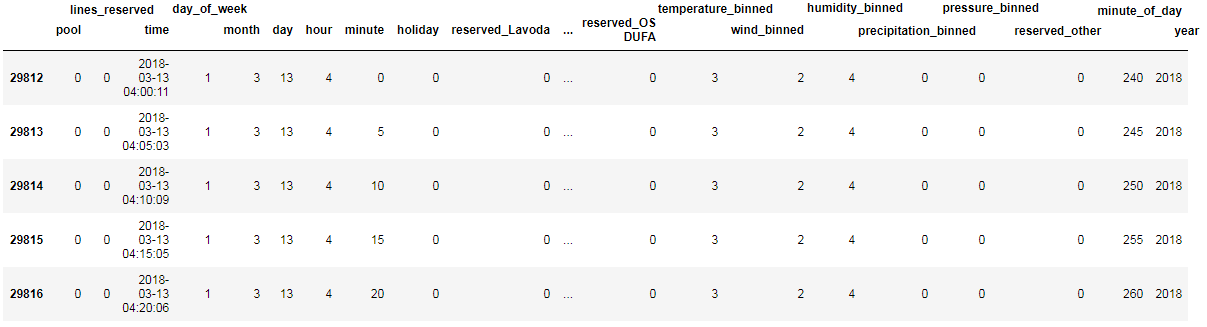
\includegraphics[width=12cm]{imgs/dataframe_head}
\caption{Structure of Data Frame after initial preprocessing and refinement that connects all available data into one table.}
\label{fig:dataframe_structure}
\end{figure}

You can see on Image \ref{fig:dataframe_structure} that only information used from \emph{occupancy} table is time stamp and pool attendance. Other data are not relevant for the occupancy of swimming pool itself. Another preprocessing step visible on Image \ref{fig:dataframe_structure} is reshaping of organisations reservation data. Database table \emph{lines\_usage} store names of organisation reserving lines in comma separated string while in this Data Frame have each organisation it's own column and value on each row represents number of lines reserved by given organisation in time stamp at that row. 


 
\color{red}
TODOs:
\begin{itemize}
    \item How DB looks - tables, image of tables
    \item Convert to CSV
    \item split of data to training testing and validation
    \item Day class 
    \item pickle of days
\end{itemize}
\color{black}

\subsection{Implementation}

\subsubsection{Monthly average - benchmark model}


\subsubsection{Random Forest Classifier}
\subsubsection{Extra Tree Classifier}
\subsubsection{Convolutional Neural Network}
Convolution Neural Network (CNN) is a type of deep learning method utilizing convolution mathematical operations. 

Throughout the implementation were tested many different models with many parameter settings. The most 
It is most commonly used f

\color{red}
TODOs:
\begin{itemize}
    \item More about CNN
    \item How is it used - cite brownlee2019cnn
    \item problems and iterations of different CNNs
\end{itemize}
\color{black}

\begin{figure}[h!]
\centering
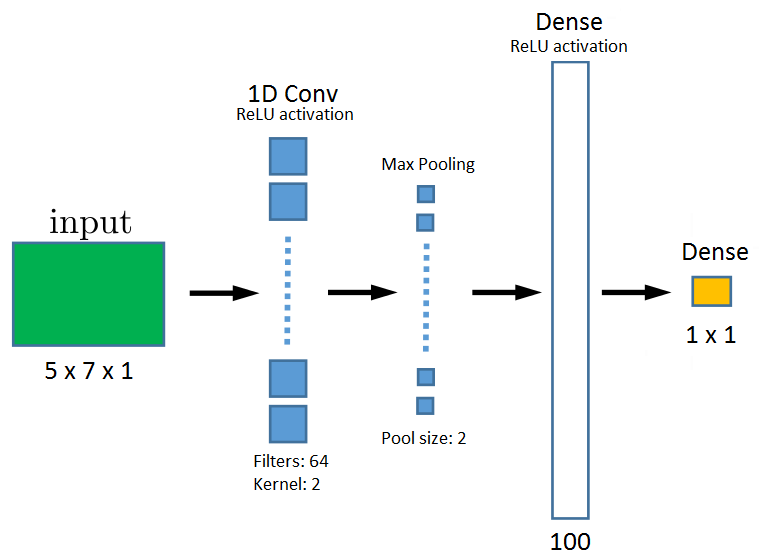
\includegraphics[width=10cm]{imgs/cnn}
\caption{Convolutional Neural Network architecture}
\label{fig:cnn}
\end{figure}


\subsubsection{Long Short Term Memory}

\color{red}
TODOs:
\begin{itemize}
    \item More about LSTM
    \item How is it used - cite brownlee2019lstm
    \item problems and iterations of different LSTM architectures, mention bidirectinal
\end{itemize}
\color{black}

\begin{figure}[h!]
\centering
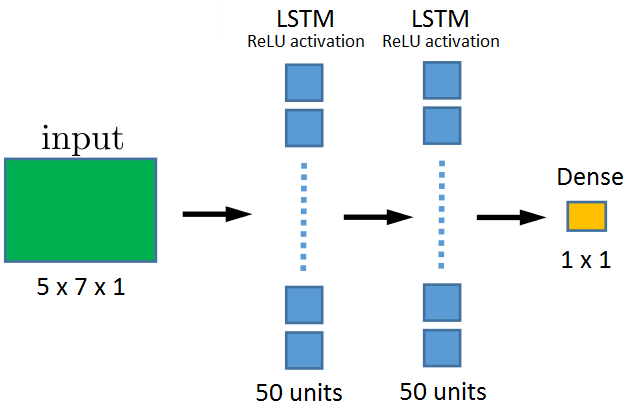
\includegraphics[width=8cm]{imgs/lstm.png}
\caption{Long Short Term Memory Network architecture}
\label{fig:lstm}
\end{figure}

\subsection{Refinement}
\subsubsection{Bin weather data}
Weather data presented large spectre of values but initial tests on Random Forests and LSTMs shows that this data had very little information gain and increase size of Random Forrest and training time of LSTMs. That is why I decide to bin weather data to followong bins:
\begin{itemize}
    \item temperature - temperature in degrees of Celsius to following 8 bins: $(-100, -5], (-5,0], (0,5], (5,10], (10,15], (15,20], (20,25], (25, 100]$
    \item wind - strength in meters per second to following 6 bins: $(-1,1], (1,5], (5,10], (10,15], (15,20], (20, 1000]$
    \item humidity - humidity in percents to following 5 bins: $(-1,20], (20,40], (40,60], (60,80], (80,100]$
    \item precipitation - rain or snow precipitation in millimeters to following 4 bins: $(-1.0,0.1], (0.1,5.0], (5.0,10.0], (10.0,1000.0]$
    \item pressure - air pressure in kPa to following 5 bins: $(0,1000], (1000,1010], (1010,1020], (1020,1030], (1030,2000]$
\end{itemize}

\subsubsection{Remove organisations with few reservations}
Encoding each organisation as new column in Data Frame with all features generated more than 100 extra columns for more than 100 organisations. But many organisations had just very few reservations and would not be beneficial to keep this information in Data Frame. That is why only organisations that regulary reserve lines and therefor their reservation could have significiant influence of overall attendance were kept in Data Frame. All the other organisations (with less than 200 reservation in total) were compressed into one column \emph{reserved\_other}. This led to reduction of number of columns to reasonable XX TODO ADD CORRECT NUMBER.

\section{Results}
\subsection{Model Evaluation and Validation}
\color{red}
TODOs:
\begin{itemize}
    \item Collect results about the performance of the models used, visualize significant quantities, and validate/justify these values. 
    \item Base results on monthly average
    \item comparisn to of monthly average to other algos
    \item influence of parameter tuning on algorithms
    \item image with MSE of all methods on testing data - bar chart
    \item image with 
\end{itemize}
\color{black}

\subsection{Justification}
\color{red}
TODOs:
\begin{itemize}
    \item Are the final results found stronger than the benchmark result reported earlier?
    \item Have you thoroughly analysed and discussed the final solution?
    \item Is the final solution significant enough to have solved the problem?
\end{itemize}
\color{black}

\section{Conclusion}

\subsection{Free-Form Visualization}
\color{red}
TODOs:
\begin{itemize}
    \item Construct conclusion about your results, and discuss whether your implementation adequately solves the problem.
    \item What was good and what bad
    \item Further improvements
\end{itemize}
\color{black}

\subsection{Reflection}

\subsection{Improvement}

\bibliographystyle{plain}
\bibliography{references}
\end{document}